\documentclass[10pt]{siamltex}
% siamltex     final
\usepackage[]{amsmath,amssymb,epsfig}
%\usepackage[]{graphicx,epsf,epsfig,amsmath,amssymb,amsfonts,latexsym,amsthm}
% \usepackage{bbm}
%\usepackage{amsfonts}
%\usepackage{amsthm}
%% \usepackage[a4paper]{geometry}
%% \geometry{top=0.99in, bottom=0.995in, left=0.995in, right=0.995in}
% \usepackage[top=20mm, bottom=18mm, left=15mm, right=18mm]{geometry}
\usepackage[top=18mm, bottom=18mm, left=20mm, right=20mm]{geometry}

\usepackage{dsfont}
\usepackage{hyperref}

% \graphicspath{{/Users/Mihai/Google Drive/MATLAB/Ranking_Sync/PLOTS/}}
% D:/LATEX/Reports@IIT/figures/
\usepackage{graphicx}
\usepackage[space]{grffile}

\newcommand{\mb}[1]{\mbox{\boldmath$#1$}}

\usepackage{url}
\usepackage{lineno}
%\pagewiselinenumbers
\usepackage{graphicx}
\usepackage{amsmath}
\usepackage{amssymb}
\usepackage{graphicx}
\usepackage{comment}
\usepackage{array}
\usepackage{algorithm}
\usepackage{algorithmic}
\usepackage{url}
\usepackage[FIGTOPCAP]{subfigure}
% \usepackage{color}

% \usepackage[toc,page]{appendix}

%\usepackage[outer]{showlabels,rotating}
%\renewcommand{\showlabelsetlabel}[1]
%{\begin{turn}{0}\showlabelfont #1\end{turn}}
%\showlabels{cite}
%\showlabels{ref}
%\showlabels{foo}
%\renewcommand{\showlabelfont}{\small}
\newtheorem{mydef}{Definition}
\newtheorem{mylem}{Lemma}
\usepackage{setspace}
\usepackage{multicol}
\usepackage{multirow}
\usepackage{color}
\usepackage{colortbl}
\usepackage{xcolor}
\usepackage{hyperref}
%\def\Acronimo{ANALYSISOFNETWORKS}
% number the lines

\newcommand{\myreferences}{../../../Postdocs_laptop/postdoc_bib_file}
% \newcommand{\myreferences}{/Users/Mihai/test_bib_file}

%\usepackage{lineno}
% \pagewiselinenumbers
%\setlength\linenumbersep{8pt}

% ANALYSISOFNETWORKS
% AALGN
\hypersetup{
%    pdftitle={\Acronimo{}, FP7-PEOPLE-IIF-2012},    % title
%    pdfauthor={Some Author},
    colorlinks=true,
    citecolor=red,
    linkcolor=blue,
    urlcolor=blue
  }

%\newtheorem{theorem}{Theorem}[section]
%\newtheorem{conjecture}[theorem]{Conjecture}
%\newtheorem{corollary}[theorem]{Corollary}
%\newtheorem{proposition}[theorem]{Proposition}
%\newtheorem{lemma}[theorem]{Lemma}
%\newdef{definition}[theorem]{Definition}
%\newdef{remark}[theorem]{Remark}
\newcounter{ale}
\newcommand{\abc}{\item[\alph{ale})]\stepcounter{ale}}
\newenvironment{liste}{\begin{itemize}}{\end{itemize}}
\newcommand{\aliste}{\begin{liste} \setcounter{ale}{1}}
\newcommand{\zliste}{\end{liste}}
\newenvironment{abcliste}{\aliste}{\zliste}

% \usepackage[english]{datetime}



\begin{document}


%\begin{pagewiselinenumbers}
\title{Implementation of the PageRank Algorithm}
\author{Justin J. Wang\footnotemark[1]  }
\date{ \today}
% \vspace{-10mm}
\maketitle
%\renewcommand{\thefootnote}{\fnsymbol{footnote}}
\footnotetext[1]{MS Data Science program, Galvanize, Inc.,  543 Howard St., San Francisco, CA 94105, email: justwjr@ucla.edu}
\footnotetext[2]{galvanizeU, 44 Tehama St., San Francisco, CA 94105, linkedin.com/in/justw; github.com/justwjr}
%\renewcommand{\thefootnote}{\arabic{footnote}}

\begin{center}
     October 11, 2016
%  DRAFT
\end{center}

% We propose novel approach to the
\vspace{5mm}

\begin{abstract}

Centrality measures are useful tools in network analysis since they quantify a node's importance in a graph modeling a network.  The definition of importance varies based on context, so choosing an appropriate centrality measure is essential. For larger networks in particular, we need to be able to find the most important nodes among hundreds or thousands of them.  PageRank centrality assigns a measure to each node based on the number of incoming edges and their weights.  It is a variant of the eigenvector centrality measure.  The algorithm is defined recursively; as a consequence, a node that has a lot of incoming edges from nodes with high PageRank has high PageRank itself.

The method was designed to rate web pages objectively and mechanically, effectively measuring the human interest and attention devoted to them.  To test the utility of PageRank for search, Brin and Page \cite{ilprints422} built a web search engine called Google.  In this paper, we apply the measure on various directed graphs from http://snap.stanford.edu/data/ - Stanford large network dataset collection.  We implement the PageRank centrality measure to order the nodes, and to see how useful it is when applied to a road network, a Facebook social network, a Google webgraph, and Amazon co-purchasing network. \cite{snapnets}  We describe the algorithm and implement it in python.

\end{abstract}


\begin{keywords} PageRank algorithm, eigenvector centrality, directed networks, graph theory
\end{keywords}


\section{Introduction}

The concept of centrality is investigated in order to answer the question, "What are the most important nodes in a network?" Centrality is an important measure used in social, biological, communication, and transportation networks since it helps analyze the relative structural prominence of nodes in the network. Especially in social network analysis it can measure the most influential or the most connected person depending on the context of the network.  PageRank was designed to rank the crawlable Web, so that web pages (nodes) with high numbers of backlinks (inedges) are deemed more important.  It is more sophisticated than simply counting number of links, which would correspond to the node degree.

\section{Centrality Measures}
Throughout the paper, we consider only the graphs $G = (V,E)$ that are simple, directed, and connected and that have $n \geq 2$ nodes. 
\subsection{Mathematical Formulation of Google PageRank}
Given a list of edges, our first step is to construct the adjacency matrix such that each cell represents the proportion of outflow from a node.  Consider the graph of a network $N = (G;c)$ with positive edge weights $c: E \rightarrow \mathbb{R}_{> 0}$ indicating the proportion of the outflow.

To illustrate, given the following graph \ref{fig:directed1} :

\begin{figure}[ht]
\begin{center}
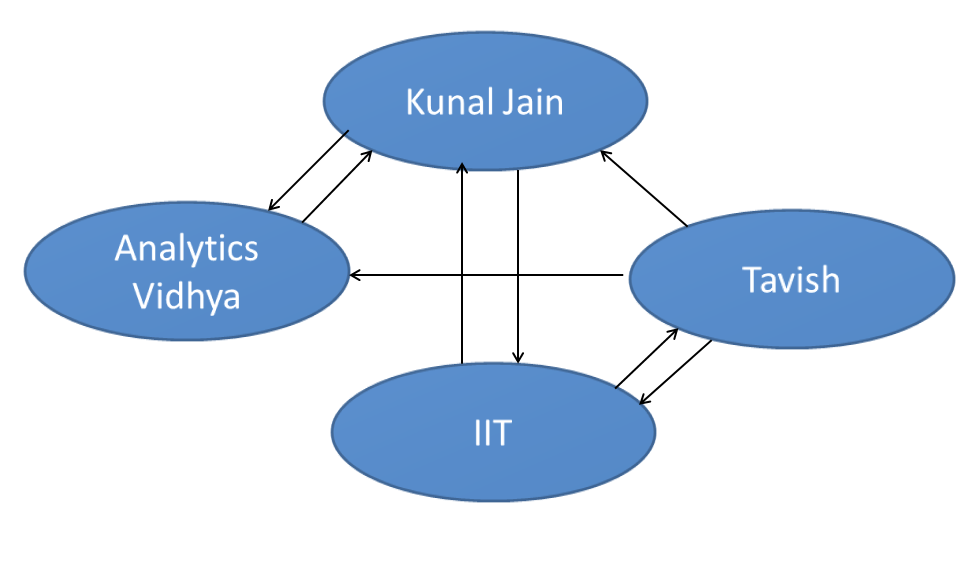
\includegraphics[width=0.56\columnwidth]{directed1}
\end{center}
\caption{Directed Graph \cite{analyticsvidhya} }
\label{fig:directed1}
\end{figure}

\vspace{5mm}
\begin{mydef}
We define the adjacency matrix $A: V \rightarrow V$ is based on the hyperlink structure of the graph.  Specifically,
\begin{align}
A_{i,j} = \frac{1}{d_i}, \text{if page i links to page j \cite{aziz2012elements}}
\end{align} where $d_i$ is the total number of unique outgoing links from page i.
\end{mydef}

Here is the corresponding adjacency matrix A for Figure \ref{fig:directed1} above:

\begin{figure}[ht]
\begin{center}
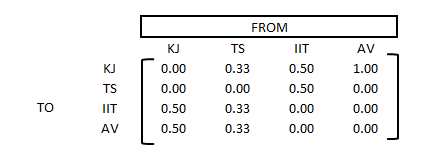
\includegraphics[width=0.56\columnwidth]{matrix1}
\end{center}
\caption{Normalized Adjacency Matrix A \cite{analyticsvidhya} }
\label{fig:matrix1}
\end{figure}
For instance, Tavish (TS) has 3 outgoing links which makes each proportion as 1/3.
\newline
Since,
\begin{align}
\sum_{j} \vec{v}_{ij} = 1 \quad \textrm{for all i}
\end{align}
and all entries are greater than or equal to 0, A is a stochastic matrix representing a transition matrix in a Markov-chain.
\newline
First, It is trivial to see that 1 is an eigenvalue of A.  In fact, the principal eigenvalue of any stochastic matrix is 1, which can be proven by contradiction or using the Gershgorin circle theorem.  The eigenvector  $\boldsymbol{\pi}$ to the eigenvalue 1 is called the stable equilibrium distribution of A. It is also called Perron-Frobenius eigenvector. \cite{knill}
\newline
Next, we construct the Markov-chain and obtain the stable equilibrium vector, $\boldsymbol{\pi}$, which is the probability vector representing the total time spent on each node.  This can be broken down into the equation:
\begin{align}
A * \boldsymbol{\pi} = \boldsymbol{\pi}
\end{align}
where $A$ is the transition matrix, and $\boldsymbol{\pi}$ is the probability of being at each transitory state.

     \subsection{Teleportation adjustments}
     Suppose we have a network $N = (G;c)$ of only 2 nodes A and B, with positive edge weights $c: E \rightarrow \mathbb{R}_{> 0}$ indicating the proportion of the outflow such that $A$ has a link to $B$ but $B$ has no external links.
     \newline
     In such cases, if you try solving the matrix, you will get a zero matrix. This looks unreasonable as B looks to be more important than A. But, our algorithm still gives same importance for both. \cite{analyticsvidhya}

To account for the end states in the Markov-chain, we introduce the concept of teleportation.  To describe the process in terms of a webgraph, we introduce a constant probability, $\boldsymbol{\epsilon}$ to each page to compensate for instances where a user teleports from one page to another without any link. \cite{analyticsvidhya}

\begin{mylem}
As a consequence, we modify our above equation with a constant $\boldsymbol{\epsilon}$:
    \begin{align}
    \boldsymbol{\pi} = \boldsymbol{\epsilon} * \vec{1} + (1 - \boldsymbol{\epsilon}) A^T \boldsymbol{\pi}
    \end{align}
    where $\vec{1}$ is a column vector of all 1s, and $\boldsymbol{\pi}[i]$ is the rank of the ith page.
\end{mylem}
\vspace{5mm}

One approach to solving the above equation is to start with a value of $\boldsymbol{\pi}$, where each component is 1/n (where n is the number of nodes) and then perform the eigenvalue/eigenvector solver on the matrix:
    \begin{align}
    A' = \boldsymbol{\epsilon} * \vec{1} + (1 - \boldsymbol{\epsilon}) A^T 
    \end{align}
    
The pseudocode for the algorithm is described below.  Also, I implemented 3 different iterative power methods, and an additional built in eigenvector solver to solving the principal eigenvector, along with their error and convergence rates, included in Appendix A \cite{eigfinder-power-methods}.

\begin{algorithm}                      % enter the algorithm environment
\caption{NumPy LAPACK Eigenvector Solver Method for PageRank \cite{hagberg-2008-exploring}}          % give the algorithm a caption
\label{alg1}                           % and a label for \ref{} commands later in the document
\begin{algorithmic}                    % enter the algorithmic environment
    \REQUIRE adjacency matrix of directed graph network $G = (V; E)$, constant teleportation probability $0 < \epsilon < 1$
\RETURN PageRank approximation $pr_{c}: V \rightarrow \mathbb{R}_{\geq 0}$, as a dictionary of nodes with PageRank as value
    \STATE n = number of rows in G
    \STATE initialize dangling weights vector of size n where each element is 1/n
    \FOR{$i=1,...,n$}
       \STATE if row sums to 0, append row index to array of dangling nodes
    \ENDFOR
    
    \FOR{$x \in dangling$ $nodes$}
    \STATE $x^{th}$ column of M = dangling weights vector
    \ENDFOR
    
   \FOR{$each$ $column \in G$}
        \FOR{each element in column}
            \STATE element /= sum(column)
        \ENDFOR
   \ENDFOR
   
   \STATE Use eigenvector solver on  $\epsilon * M + (1 - \epsilon) * dangling weights$ to obtain principal eigenvector
    \STATE sort eigenvalues to obtain index of principal eigenvector
    \RETURN normalized principal eigenvector

\end{algorithmic}
\end{algorithm}

\section{History}
In 1976 by Pinski and Narin suggested the eigenvalue problem while working on scientometrics ranking scientific journals.  Page and Brin developed PageRank at Stanford in 1996 as part of search engine research.  Brin had the idea of "link popularity".  They and two others published a paper in 1998, cited below. \cite{ilprints422}

In practice, Google does not rely solely on PageRank.  On October 15, 2009, a Google employee confirmed that the company had removed PageRank from its Webmaster Tools section, saying that "We've been telling people for a long time that they shouldn't focus on PageRank so much.  On April 15, 2016 Google has officially shut down their Google Toolbar PageRank Data to public. Google had told about this earlier that they would be removing the PageRank score from the google toolbar months before in advance.  As of writing, the top 3 metrics are Links, Content,, and RankBrain.  PageRank is deprecated.\cite{wiki:PageRank}

\section{Current Uses}
\label{sec:uses_and_history}
Besides its originally designed purpose to rank websites, PageRank is now regularly used in bibliometrics, social and information network analysis, and for link prediction and recommendation. It's even used for systems analysis of road networks, as well as biology, chemistry, neuroscience, and physics. 

Twitter uses Personal PageRank to present users with other accounts they may wish to follow.

Another is to rank academic doctoral programs based on their records of placing their graduates in faculty positions. In PageRank terms, academic departments link to each other by hiring their faculty from each other (and from themselves).

In a road network, it's used to rank spaces or streets to predict how many people (pedestrians or vehicles) come to the individual spaces or streets.  Pagerank has recently been used to quantify the scientific impact of researchers, through the citation and collaboration networks \cite{wiki:PageRank}

\section{Summary and conclusion}  \label{sec:conclusion}
%Summarize your work in this section.
The applications of PageRank are not limited to webpages, rather, the centrailty measure can be applied to any network that can be represented as a directed graph of nodes and edges.  In particular, the algorithm can be applied to social networks to quantify how important a person is compared to everyone else.  Similarly, we can run the process through data of a road network or Amazon's co-purchasing network.

\begin{figure}[ht]
\begin{center}
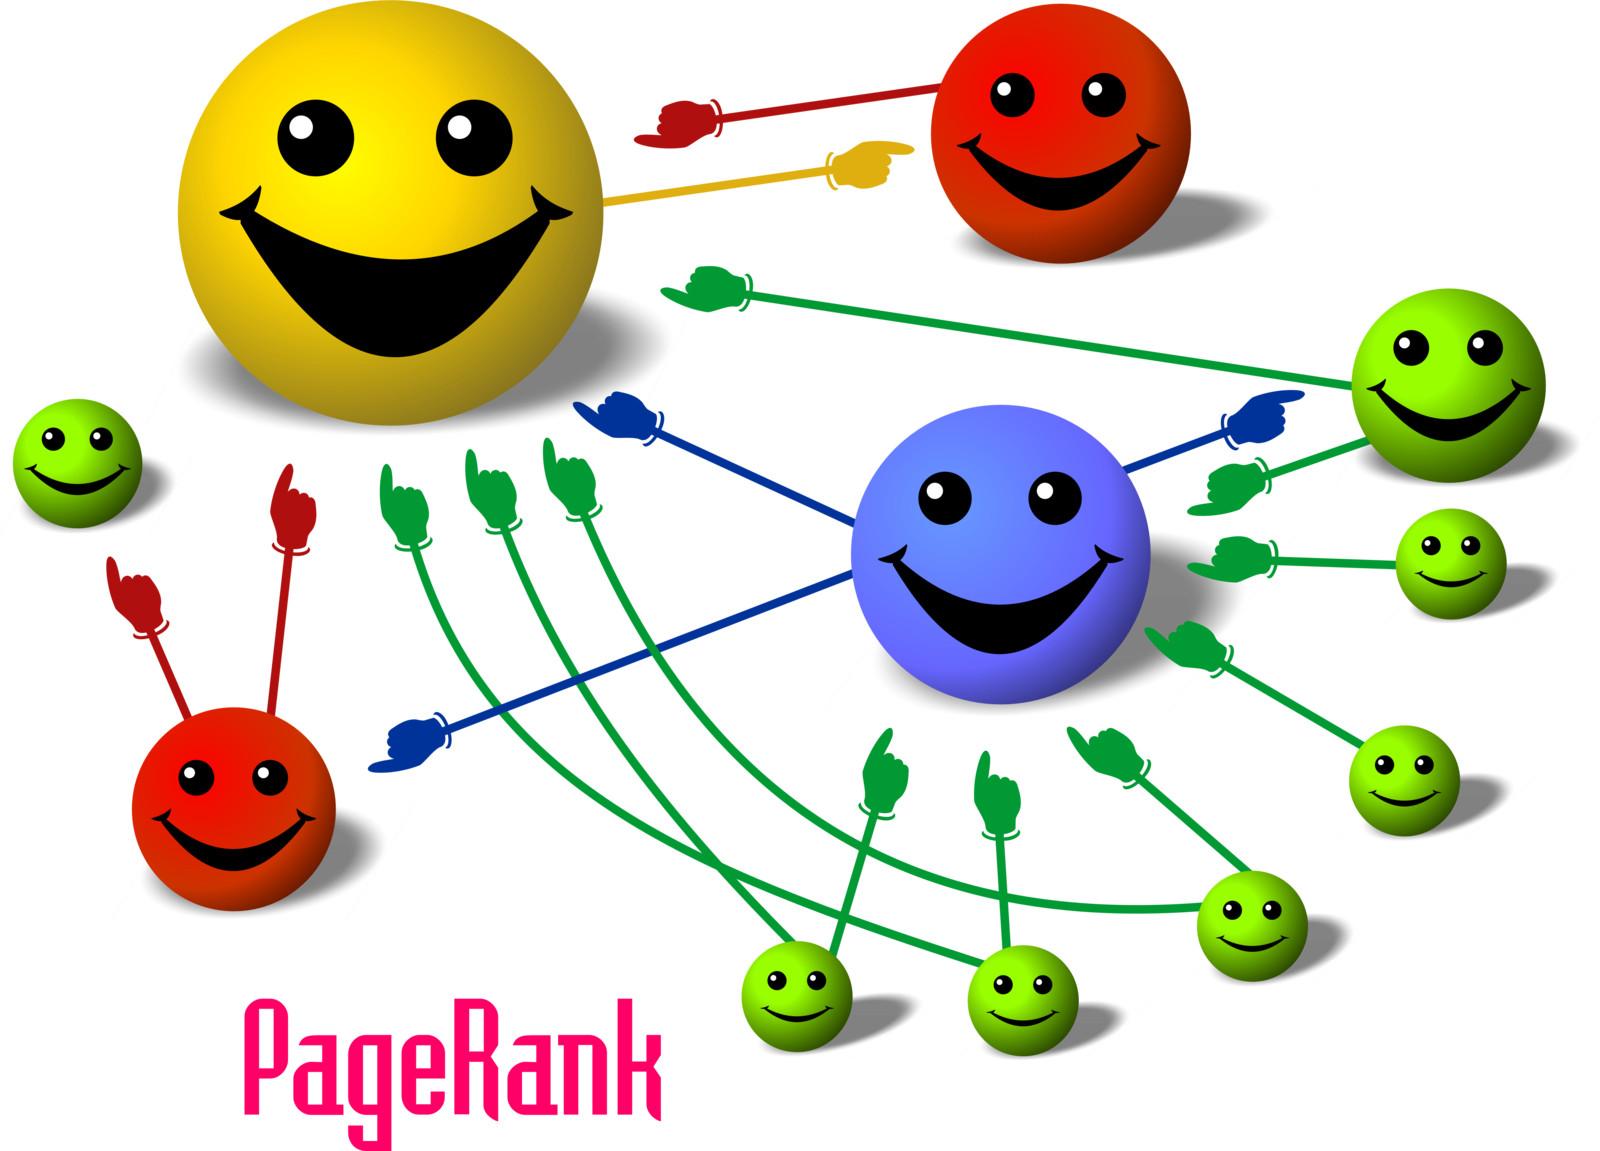
\includegraphics[width=0.4\columnwidth]{PageRank-hi-res}
\end{center}
\caption{Size Proportional Smilies\cite{wiki:PageRank} }
\label{fig:PageRank-hi-res}
\end{figure}

\newpage
\bibliographystyle{siam}
\bibliography{bibliography}

%\end{pagewiselinenumbers}

\end{document}